%===============================================================================
% LaTeX sjabloon voor de bachelorproef toegepaste informatica aan HOGENT
% Meer info op https://github.com/HoGentTIN/latex-hogent-report
%===============================================================================

\documentclass[dutch,dit,thesis]{hogentreport}

% TODO:
% - If necessary, replace the option `dit`' with your own department!
%   Valid entries are dbo, dbt, dgz, dit, dlo, dog, dsa, soa
% - If you write your thesis in English (remark: only possible after getting
%   explicit approval!), remove the option "dutch," or replace with "english".

\usepackage{lipsum} % For blind text, can be removed after adding actual content

%% Pictures to include in the text can be put in the graphics/ folder
\graphicspath{{graphics/}}

%% For source code highlighting, requires pygments to be installed
%% Compile with the -shell-escape flag!
\usepackage[section]{minted}
\usemintedstyle{solarized-light}
\definecolor{bg}{RGB}{253,246,227} %% Set the background color of the codeframe

%% Change this line to edit the line numbering style:
\renewcommand{\theFancyVerbLine}{\ttfamily\scriptsize\arabic{FancyVerbLine}}

%% Macro definition to load external java source files with \javacode{filename}:
\newmintedfile[javacode]{java}{
    bgcolor=bg,
    fontfamily=tt,
    linenos=true,
    numberblanklines=true,
    numbersep=5pt,
    gobble=0,
    framesep=2mm,
    funcnamehighlighting=true,
    tabsize=4,
    obeytabs=false,
    breaklines=true,
    mathescape=false
    samepage=false,
    showspaces=false,
    showtabs =false,
    texcl=false,
}

% Other packages not already included can be imported here

%%---------- Document metadata -------------------------------------------------
% TODO: Replace this with your own information
\author{Jona De Neve}
\supervisor{Mevr. Lena De Mol}
\cosupervisor{Mevr. Jana Van Damme}
\title[]%
    {Verbeteren van VR stottertherapie door het herkennen en verwerken van verbale antwoorden met spraakherkenningssoftware}
\academicyear{\advance\year by -1 \the\year--\advance\year by 1 \the\year}
\examperiod{2}
\degreesought{\IfLanguageName{dutch}{Professionele bachelor in de toegepaste informatica}{Bachelor of applied computer science}}
\partialthesis{false} %% To display 'in partial fulfilment'
%\institution{Internshipcompany BVBA.}

%% Add global exceptions to the hyphenation here
\hyphenation{back-slash}

%% The bibliography (style and settings are  found in hogentthesis.cls)
\addbibresource{bachproef.bib}            %% Bibliography file
\addbibresource{../voorstel/voorstel.bib} %% Bibliography research proposal
\defbibheading{bibempty}{}

%% Prevent empty pages for right-handed chapter starts in twoside mode
\renewcommand{\cleardoublepage}{\clearpage}

\renewcommand{\arraystretch}{1.2}

%% Content starts here.
\begin{document}

%---------- Front matter -------------------------------------------------------

\frontmatter

\hypersetup{pageanchor=false} %% Disable page numbering references
%% Render a Dutch outer title page if the main language is English
\IfLanguageName{english}{%
    %% If necessary, information can be changed here
    \degreesought{Professionele Bachelor toegepaste informatica}%
    \begin{otherlanguage}{dutch}%
       \maketitle%
    \end{otherlanguage}%
}{}

%% Generates title page content
\maketitle
\hypersetup{pageanchor=true}

%%=============================================================================
%% Voorwoord
%%=============================================================================

\chapter*{\IfLanguageName{dutch}{Woord vooraf}{Preface}}%
\label{ch:voorwoord}

%% TODO:
%% Het voorwoord is het enige deel van de bachelorproef waar je vanuit je
%% eigen standpunt (``ik-vorm'') mag schrijven. Je kan hier bv. motiveren
%% waarom jij het onderwerp wil bespreken.
%% Vergeet ook niet te bedanken wie je geholpen/gesteund/... heeft

Deze bachelorproef werd geschreven in het kader van het voltooien van de opleiding Toegepaste Informatica afstudeerrichting Mobile \& Enterprise development. Hoewel dit onderwerp niet valt onder mijn afstudeerrichting, koos ik ervoor uit interesse van de huidige stand van Artificiële Intelligentie en hoe het verder evolueert in de toekomst. Zo volg ik de vooruitgang ook wekelijks. Daarnaast wil ik graag een aantal mensen bedanken, zonder wie deze proef niet tot stand zou zijn gekomen.

In de eerste plaats wil ik mijn co-promotor, Jana Van Damme, bedanken voor de hulp tijdens de opzet van deze bachelorproef en voor alle nuttige feedback onderweg.

Daarnaast wil ik mijn promotor, Lena De Mol, bedanken voor

%%=============================================================================
%% Samenvatting
%%=============================================================================

% TODO: De "abstract" of samenvatting is een kernachtige (~ 1 blz. voor een
% thesis) synthese van het document.
%
% Een goede abstract biedt een kernachtig antwoord op volgende vragen:
%
% 1. Waarover gaat de bachelorproef?
% 2. Waarom heb je er over geschreven?
% 3. Hoe heb je het onderzoek uitgevoerd?
% 4. Wat waren de resultaten? Wat blijkt uit je onderzoek?
% 5. Wat betekenen je resultaten? Wat is de relevantie voor het werkveld?
%
% Daarom bestaat een abstract uit volgende componenten:
%
% - inleiding + kaderen thema
% - probleemstelling
% - (centrale) onderzoeksvraag
% - onderzoeksdoelstelling
% - methodologie
% - resultaten (beperk tot de belangrijkste, relevant voor de onderzoeksvraag)
% - conclusies, aanbevelingen, beperkingen
%
% LET OP! Een samenvatting is GEEN voorwoord!

%%---------- Nederlandse samenvatting -----------------------------------------
%
% TODO: Als je je bachelorproef in het Engels schrijft, moet je eerst een
% Nederlandse samenvatting invoegen. Haal daarvoor onderstaande code uit
% commentaar.
% Wie zijn bachelorproef in het Nederlands schrijft, kan dit negeren, de inhoud
% wordt niet in het document ingevoegd.

\IfLanguageName{english}{%
\selectlanguage{dutch}
\chapter*{Samenvatting}
%\lipsum[1-4]
\selectlanguage{english}
}{}

%%---------- Samenvatting -----------------------------------------------------
% De samenvatting in de hoofdtaal van het document

\chapter*{\IfLanguageName{dutch}{Samenvatting}{Abstract}}



%---------- Inhoud, lijst figuren, ... -----------------------------------------

\tableofcontents

% In a list of figures, the complete caption will be included. To prevent this,
% ALWAYS add a short description in the caption!
%
%  \caption[short description]{elaborate description}
%
% If you do, only the short description will be used in the list of figures

\listoffigures

% If you included tables and/or source code listings, uncomment the appropriate
% lines.
%\listoftables
%\listoflistings

% Als je een lijst van afkortingen of termen wil toevoegen, dan hoort die
% hier thuis. Gebruik bijvoorbeeld de ``glossaries'' package.
% https://www.overleaf.com/learn/latex/Glossaries

%---------- Kern ---------------------------------------------------------------

\mainmatter{}

% De eerste hoofdstukken van een bachelorproef zijn meestal een inleiding op
% het onderwerp, literatuurstudie en verantwoording methodologie.
% Aarzel niet om een meer beschrijvende titel aan deze hoofdstukken te geven of
% om bijvoorbeeld de inleiding en/of stand van zaken over meerdere hoofdstukken
% te verspreiden!

%%=============================================================================
%% Inleiding
%%=============================================================================

\chapter{\IfLanguageName{dutch}{Inleiding}{Introduction}}%
\label{ch:inleiding}

In de reclamespot `The Impact Will Be Real` over de Metaverse toont \textcite{Meta2022} hun visie over de rol die Virtual Reality (VR) speelt in de toekomst. Zo laten ze verschillende toepassingen ervan in het onderwijs zien. Jammer genoeg staat onze technologie nog niet zo ver als wat er in de reclame gezien kan worden maar ook nu al vindt VR zich een baan in verschillende opleidingen.

De Hogeschool van Gent maakt ook gebruik van VR om studenten de kans te geven in meer realistische situaties te oefenen. Hiervoor zijn twee verschillende technieken gebruikt. Allereerst heb je het renderen van een omgeving. Dit laat de gebruiker een interactieve wereld van 3D modellen ontdekken. Zo bestaan er drie virtuele kamers waarin de student kan oefenen. De andere manier is aan de hand van een 360° opname die wordt gemaakt aan de hand van een 360° camera. Omdat dit een opname van de werkelijkheid neemt, ziet deze methode er realistischer uit.

Dit is waar er op het probleem wordt gestoten. Aangezien de tweede methode werkt met een opname moet er naar verschillende fragmenten gesprongen worden naargelang het antwoord dat de gebruiker ingeeft. Dit wordt handmatig gedaan door een begeleider. Hierdoor staat de oefening tijdelijk stil wat de echtheid van de situatie weghaalt. Daarom wordt in deze bachelorproef toegepaste informatica onderzocht hoe het overschakelen anders kan aangepakt worden zodat het voor de gebruiker realistischer aanvoelt. Hiervoor kijken we richting Artificiële Intelligentie (AI).

Het afgelopen jaar is de populariteit van AI enorm gestegen. Van text-to-image models zoals DALL-E 2, Imagen en Stable diffusion die een gegeven tekst prompt kunnen omzetten in afbeeldingen tot voice-models die stemmen kunnen imiteren, zo goed als iedereen heeft al gehoord van AI. Meestal is het jammer genoeg het negatieve aan AI dat de ronde doet zoals het verspreiden van misinformatie aan de hand van deepfakes of het schenden van auteursrechten maar afgezien dat heeft het veel mogelijk heden om de mensheid te helpen.


%De inleiding moet de lezer net genoeg informatie verschaffen om het onderwerp te begrijpen en in te zien waarom de onderzoeksvraag de moeite waard is om te onderzoeken. In de inleiding ga je literatuurverwijzingen beperken, zodat de tekst vlot leesbaar blijft. Je kan de inleiding verder onderverdelen in secties als dit de tekst verduidelijkt. Zaken die aan bod kunnen komen in de inleiding~\autocite{Pollefliet2011}:
%
%\begin{itemize}
%  \item context, achtergrond
%  \item afbakenen van het onderwerp
%  \item verantwoording van het onderwerp, methodologie
%  \item probleemstelling
%  \item onderzoeksdoelstelling
%  \item onderzoeksvraag
%  \item \ldots
%\end{itemize}

\section{\IfLanguageName{dutch}{Probleemstelling}{Problem Statement}}%
\label{sec:probleemstelling}

Wanneer de stotterpatiënt antwoordt op de gestelde vraag wordt er niet automatisch overgeschakeld naar een volgend fragment. Er moet namelijk handmatig geklikt worden op het gewenste hoofdstuk door iemand die de oefening kent. Dit zorgt dat er steeds een begeleider aanwezig moet zijn. Ook zal de dynamiek van de oefening verbroken worden omdat het pas verder kan gaan wanneer de begeleider het juiste fragment vindt.

%Uit je probleemstelling moet duidelijk zijn dat je onderzoek een meerwaarde heeft voor een concrete doelgroep. De doelgroep moet goed gedefinieerd en afgelijnd zijn. Doelgroepen als ``bedrijven,'' ``KMO's'', systeembeheerders, enz.~zijn nog te vaag. Als je een lijstje kan maken van de personen/organisaties die een meerwaarde zullen vinden in deze bachelorproef (dit is eigenlijk je steekproefkader), dan is dat een indicatie dat de doelgroep goed gedefinieerd is. Dit kan een enkel bedrijf zijn of zelfs één persoon (je co-promotor/opdrachtgever).

\section{\IfLanguageName{dutch}{Onderzoeksvraag}{Research question}}%
\label{sec:onderzoeksvraag}

Om dit probleem te verhelpen wordt hiervoor gekeken hoe AI te hulp kan schieten om stotterpatiënten een meer interactieve ervaring geven. Om dit te realiseren zullen de volgende vragen beantwoord worden:
\begin{itemize}
    \item Hoe gaat de applicatie registreren wat er werd gezegd?
    \item Wat kan er mislopen bij het registreren van spraak?
    \item Welke aspecten van stotteren hebben effect op de spraakherkenning?
    \item Hoe kiest de applicatie een volgend fragment op basis van de gegenereerde tekst?
\end{itemize}

%Wees zo concreet mogelijk bij het formuleren van je onderzoeksvraag. Een onderzoeksvraag is trouwens iets waar nog niemand op dit moment een antwoord heeft (voor zover je kan nagaan). Het opzoeken van bestaande informatie (bv. ``welke tools bestaan er voor deze toepassing?'') is dus geen onderzoeksvraag. Je kan de onderzoeksvraag verder specifiëren in deelvragen. Bv.~als je onderzoek gaat over performantiemetingen, dan

\section{\IfLanguageName{dutch}{Onderzoeksdoelstelling}{Research objective}}%
\label{sec:onderzoeksdoelstelling}

In deze bachelorproef wordt een proof of concept opgesteld om te kijken hoe zo een AI-applicatie te werk zou kunnen gaan. De bedoeling van deze applicatie is eerst en vooral het registreren wanneer de gebruiker aan het antwoorden is. Vervolgens transcribeert het wat er gezegd wordt. Als laatste gaat het op basis van de context een gepast fragment zoeken om verder mee te gaan.

%Wat is het beoogde resultaat van je bachelorproef? Wat zijn de criteria voor succes? Beschrijf die zo concreet mogelijk. Gaat het bv.\ om een proof-of-concept, een prototype, een verslag met aanbevelingen, een vergelijkende studie, enz.

\section{\IfLanguageName{dutch}{Opzet van deze bachelorproef}{Structure of this bachelor thesis}}%
\label{sec:opzet-bachelorproef}

% Het is gebruikelijk aan het einde van de inleiding een overzicht te
% geven van de opbouw van de rest van de tekst. Deze sectie bevat al een aanzet
% die je kan aanvullen/aanpassen in functie van je eigen tekst.

De rest van deze bachelorproef is als volgt opgebouwd:

In Hoofdstuk~\ref{ch:stand-van-zaken} wordt een overzicht gegeven van de stand van zaken binnen het onderzoeksdomein, op basis van een literatuurstudie.

In Hoofdstuk~\ref{ch:methodologie} wordt de methodologie toegelicht en worden de gebruikte onderzoekstechnieken besproken om een antwoord te kunnen formuleren op de onderzoeksvragen.

% TODO: Vul hier aan voor je eigen hoofdstukken, één of twee zinnen per hoofdstuk
In Hoofdstuk~\ref{ch:resultaten} worden de resultaten besproken.

In Hoofdstuk~\ref{ch:conclusie}, tenslotte, wordt de conclusie gegeven en een antwoord geformuleerd op de onderzoeksvragen. Daarbij wordt ook een aanzet gegeven voor toekomstig onderzoek binnen dit domein.
\chapter{\IfLanguageName{dutch}{Stand van zaken}{State of the art}} \label{chap:State of the art}%
\label{ch:stand-van-zaken}

% Tip: Begin elk hoofdstuk met een paragraaf inleiding die beschrijft hoe
% dit hoofdstuk past binnen het geheel van de bachelorproef. Geef in het
% bijzonder aan wat de link is met het vorige en volgende hoofdstuk.

% Pas na deze inleidende paragraaf komt de eerste sectiehoofding.

Zoals vermeld in de inleiding heeft het zorglab van Hogeschool Gent verschillende doeleinden. Zo kunnen studenten geneeskunde leren hoe ze een operatie moeten uitvoeren zonder iemand als testpersoon te gebruiken. Anderzijds kan het een persoon die plankenkoorts heeft een presentatie of een toespraak leren houden. In onze situatie zal een patiënt met een stotter leren een vlot gesprek te houden zoals bijvoorbeeld wanneer hij op sollicitatie gaat. Dit wordt gerealiseerd aan de hand van 360° opnames die voor de patiënt opnieuw afgespeeld kunnen worden in VR.

\section{\IfLanguageName{dutch}{Virtuele realiteit}{Virtual reality}}%
Hoewel Virtual Reality tegenwoordig veel gevorderd is, bestaat het al voor een lange tijd. Het eerste toestel dat de werkelijkheid nabootste was Morton Heilig’s Sensorama uit 1962. Dit liet de gebruiker ervaren hoe het voelde om op een motor door Boston te rijden. De opvolgende jaren werden ook andere toestellen uitgevonden zoals de 'Sword of Damocles' die de locatie van het hoofd en de ogen volgde en Nintendo's 'power glove' voor de NES \autocite{Boas2012}.

De eerste vermelding van de term VR daarentegen kwam pas rond 1985 zegt \textcite{Bryson2013}. Hij verteld over hoe Jaron Lanier de term 'virtual reality' gebruikte om het Virtual Interactive Environment Workstation (VIEW) lab van NASA te beschrijven. De daaropvolgende jaren werd de term steeds populairder met als gevolg dat het ruim werd toegepast op verschillende toepassingen. Daarom moest de term VR goed gedefinieerd worden:

\begin{quote}
    Virtual Reality is the use of computer technology to create the effect of an
    interactive three-dimensional world in which the objects have a sense of spatial
    presence. \autocite{Bryson2013}
\end{quote}

Tegenwoordig zijn VR toestellen te vinden in vele soorten een maten. Zo zijn er headsets gemaakt voor PC of consoles en anderen voor smartphones. Dankzij software en hardware verbeteringen bestaan er nu zelfs headsets die autonoom werken. Dit zorgt ervoor dat kabels en complexe set-ups niet nodig zijn. Deze verbeteringen zorgen ook dat de digitale wereld realistischer doet aanvoelen.

\section{\IfLanguageName{dutch}{Artificiële intelligentie}{Artificial intelligence}}%
Het afgelopen jaar is de populariteit van AI enorm gestegen. Met text-to-image models zoals DALL-E 2, Imagen en Stable diffusion die een gegeven tekst prompt kunnen omzetten in afbeeldingen. Daarnaast zijn er ook applicaties die language models gebruiken zoals Chat-GPT, spraak assistenten en Github Copilot. Zij kunnen teksten verwerken en accurate antwoorden genereren op basis van hun kennis ook al zijn deze niet altijd accuraat (Meer hierover in \ref{ssec:Natural Language Classifier})

Om het overschakelen naar een volgend fragment te laten gebeuren zonder begeleiding en zonder veel tijd te verliezen, zouden verbale antwoorden gegeven kunnen worden. Een mooi voorbeeld van een gelijkaardige interactie is het project 'Dimensions in Testimony' van de \textcite{USCShoahFoundation2020}. Daar kunnen bezoekers vragen stellen aan een overlevende van de Holocaust die op voorhand een volledig interview heeft afgelegd. Dit werd mogelijk gemaakt dankzij het systeem dat erachter zit (Figuur \ref{fig:DiTArchitecture}). Dit systeem is opgebouwd uit volgende componenten: een software voor spraakherkenning (ASR) die de gebruikers verbale vraag in tekst omzet, een Natural Language Classifier (NLC) die op basis van de gegenereerde tekst een antwoord via een audio/video fragment voorziet en een mediaspeler die de fragmenten kan afspelen met tussendoor een inactieve animatie \autocite{Traum2015}.

\begin{figure}[h]
    \centering
    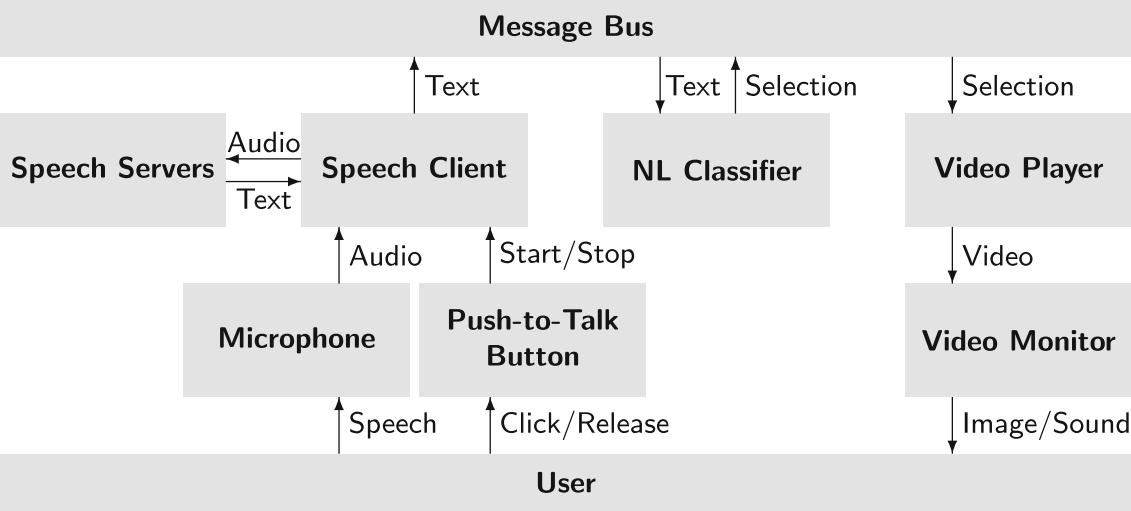
\includegraphics[width=\linewidth*3/4]{TraumDEtAl_DimensionsInTestimony_SystemArchitecture.png}
    \caption{Dimensions in Testimony - Systeem Architectuur \autocite{Traum2015}}
    \label{fig:DiTArchitecture}
\end{figure}

Een ander voorbeeld zijn de home assistenten zoals Google Home, Amazon Echo of Apple HomePod. Zij staan op stand-by tot de gebruiker het triggerwoord zegt, `Hey Google' bijvoorbeeld. Eenmaal geactiveerd luisteren ze naar wat de gebruiker zegt en zetten ze dit aan de hand van een ASR om naar tekst. Daarna haalt het met natuurlijke taalverwerking (NLP) de intentie en sleutelwoorden uit de tekst en genereert daarmee een gepast antwoord. Als laatste zet het gegenereerde tekst om naar spraak.

\subsection{\IfLanguageName{dutch}{Spraakherkening}{Speech recognition}}%

Net als VR is spraakherkenning de laatste jaren veel vooruitgegaan, dit komt omdat er meer data beschikbaar is, de computers sneller en de algoritmes, genaamd deep neural networks, beter zijn. Deze netwerken worden getraind op grote datasets bestaande uit diverse spraakfragmenten. Hieruit leert het de patronen en kenmerken van menselijke spraak.

Maar perfect zullen ze nooit zijn zegt \textcite{Hessen2020}. Dit is geen verrassing aangezien zelf mensen vaak nog problemen hebben bij het verstaan van een andere. De meest voorkomende fouten van een ASR zijn herkenningsfouten. Deze kunnen ontstaan door slechte kwaliteit van de opname maar ook van de manier waarop woorden worden uitgesproken. De andere fouten ontstaan omdat ASR zijn vocabulaire niet uitgebreid genoeg is. Dit noemen we Out-of-vocabulary-fouten (OOV) \autocite{Hessen2020}.



\subsection{\IfLanguageName{dutch}{Natuurlijke taalverwerking}{Natural Language Classifier}} \label{ssec:Natural Language Classifier}%

Naast de ASR hebben we ook de natuurlijke taalverwerking (NLP). In 'Dimension in Testimony' maakten ze hiervoor gebruik van NCPEditor (Figuur \ref{fig:NPCEArchitecture}). De classifier in dit systeem berekent welke antwoorden op de ingegeven tekst kunnen gegeven worden door de taalmodellen van beide te vergelijken en de antwoorden te rangschikken. Zolang de ingegeven tekst een foutmarge lager dan 50\% blijft, zal het antwoord ongewijzigd blijven \autocite{Leuski2010}.

Een andere bekend taalmodel is GPT-3. Dit model ligt aan de basis van de populaire chatbot ChatGPT.

\begin{figure}[h]
    \centering
    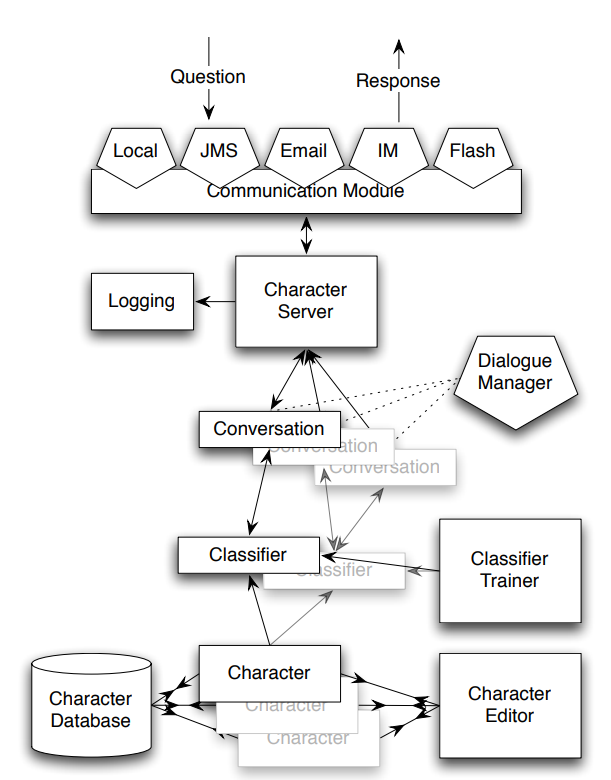
\includegraphics[width=\linewidth*3/4]{Traum&Leuski_NPCEditor_System architecture.png}
    \caption{NPCEditor - Systeem Architectuur \autocite{Leuski2010}}
    \label{fig:NPCEArchitecture}
\end{figure}



\chapter{\IfLanguageName{dutch}{Long list}{Long list}} \label{chap:Long list}%
\label{ch:long-list}

\section{\IfLanguageName{dutch}{Spraakherkening}{Speech recognition}}\label{sec:Speech recognition}%

\subsection{Google Cloud Speech-to-text API}%

Google Cloud Speech-to-text API is Google's kijk op spraakherkennigssoftware. Hun service kan per maand 60 minuten gratis gebruikt worden. Daarna moet er per minuut van €0,016 voor standaard met datalogging tot €0,072 voor medisch gebruik zonder datalogging. De service komt ook met verschillende functies zoals het automatisch detecteren van de gesproken taal, het herkennen van verschillende stemmen en real-time streaming om live spraak naar tekst om te zetten.

De API is ook heel betrouwbaar. Zo heeft een succespercentage van 100\% voor normale stemmen en een percentage tussen 83,3\% en 90\% voor mensen met een spraakbeperking \autocite{Anggraini2018}. Daarnaast bied het ook de mogelijkheid om het model uit te breiden door het nieuwe vocabulaire aan te leren.


\subsection{Amazon Transcribe}%

Ook Amazon Web Services (AWS) bied een ASR software aan genaamd Amazon Transcribe. Het bied net als Google's ASR ook een aantal feautures aan zoals herkennen van verschillende stemmen, vocabulaire uitbreiden met jargon van het gewenste doeleinden toevoegen van eigen modellen en real-time transcriptie. De laatste twee functies zijn wel niet beschikbaar in het Nederlands. De service kan 60 minuten per maand gratis gebruikt worden, gedurende 12 maanden. Daarna moet er een vergoeding worden betaald afhankelijk van het totale gebruik per maand en de geolocatie van de gebruikte server (Figuur \ref{fig:PricingAmazonTranscribe}).

\begin{figure}[h]
    \centering
    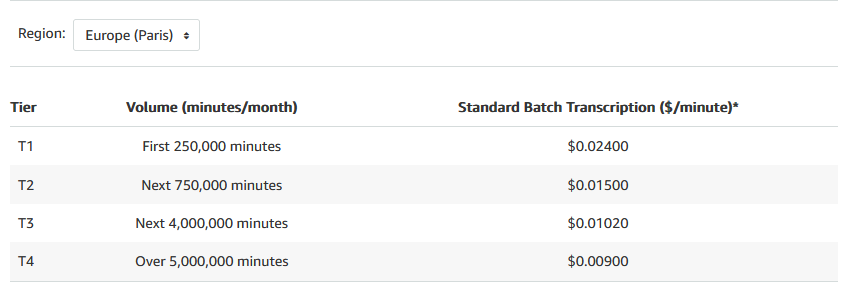
\includegraphics[width=\linewidth*3/4]{graphics/AmazonTranscribePricing.png}
    \caption{Prijzen Amazon Transcribe voor Parijse server \autocite{Amazon2023}}
    \label{fig:PricingAmazonTranscribe}
\end{figure}

\subsection{Microsoft Azure Speech Services}%

Microsoft Azure Speech Services

\subsection{Mozilla Deepspeech}%

test

\subsection{Whisper}%

Whisper is OpenAI's


\section{\IfLanguageName{dutch}{Natuurlijke taalverwerking}{Natural Language Classifier}} \label{sec:Natural Language Classifier}%

%Dit hoofdstuk bevat je literatuurstudie. De inhoud gaat verder op de inleiding, maar zal het onderwerp van de bachelorproef *diepgaand* uitspitten. De bedoeling is dat de lezer na lezing van dit hoofdstuk helemaal op de hoogte is van de huidige stand van zaken (state-of-the-art) in het onderzoeksdomein. Iemand die niet vertrouwd is met het onderwerp, weet nu voldoende om de rest van het verhaal te kunnen volgen, zonder dat die er nog andere informatie moet over opzoeken \autocite{Pollefliet2011}.
%
%Je verwijst bij elke bewering die je doet, vakterm die je introduceert, enz.\ naar je bronnen. In \LaTeX{} kan dat met het commando \texttt{$\backslash${textcite\{\}}} of \texttt{$\backslash${autocite\{\}}}. Als argument van het commando geef je de ``sleutel'' van een ``record'' in een bibliografische databank in het Bib\LaTeX{}-formaat (een tekstbestand). Als je expliciet naar de auteur verwijst in de zin, gebruik je \texttt{$\backslash${}textcite\{\}}.
%Soms wil je de auteur niet expliciet vernoemen, dan gebruik je \texttt{$\backslash${}autocite\{\}}. In de volgende paragraaf een voorbeeld van elk.
%
%\textcite{Knuth1998} schreef een van de standaardwerken over sorteer- en zoekalgoritmen. Experten zijn het erover eens dat cloud computing een interessante opportuniteit vormen, zowel voor gebruikers als voor dienstverleners op vlak van informatietechnologie~\autocite{Creeger2009}.
%
%\lipsum[7-20]

\chapter{\IfLanguageName{dutch}{Long list}{Long list}} \label{chap:Long list}%
\label{ch:long-list}

\section{\IfLanguageName{dutch}{Spraakherkening}{Speech recognition}}\label{sec:Speech recognition}%

\subsection{Google Cloud Speech-to-text API}%

\paragraph{\IfLanguageName{dutch}{Beschrijving}{Description}}
Google Cloud Speech-to-text API is Google's kijk op spraakherkennigssoftware. De API is heel betrouwbaar. Zo heeft het volgens \textcite{Anggraini2018} een succespercentage van 100\% voor normale stemmen en een percentage tussen 83,3\% en 90\% voor mensen met een spraakbeperking. Daarnaast bied het ook de mogelijkheid om het model uit te breiden door het nieuwe vocabulaire aan te leren.

\paragraph{\IfLanguageName{dutch}{Functies}{Features}}
De service komt met verschillende functies. Dit zijn de belangrijke kenmerken die ze adverteren:

\begin{itemize}
    \item \textbf{Taalherkenning}: De API ondersteunt spraakherkenning in verschillende talen en dialecten, waardoor gebruikers wereldwijd toegang hebben tot de dienst. Het kan automatisch de gesproken taal detecteren zonder voorafgaande taalconfiguratie.

    \item \textbf{Real-time streaming}: De API ondersteunt real-time streaming van spraak naar tekst, waardoor ontwikkelaars toepassingen kunnen bouwen die directe feedback en interactie vereisen, zoals live ondertiteling, spraakgestuurde commando's en real-time transcriberen.

    \item \textbf{Hoge nauwkeurigheid}: Dankzij de geavanceerde neurale netwerkmodellen levert de Speech-to-Text API nauwkeurige transcripties, zelfs in omgevingen met achtergrondgeluiden, verschillende spreekstijlen en spraak van meerdere sprekers.

    \item \textbf{Aanpasbare modellen}: Gebruikers kunnen de spraakherkenning aanpassen aan specifieke woordenschat en domeinen door aangepaste woordenlijsten en grammatica's te gebruiken. Dit verhoogt de nauwkeurigheid en zorgt voor een betere herkenning van vakspecifieke terminologie.

    \item \textbf{Multimediaondersteuning}: De API kan spraak herkennen in verschillende formaten, waaronder audio-opnamen, audiobestanden en streaming-audio. Dit maakt integratie met verschillende bronnen en toepassingen mogelijk.

    \item \textbf{Beveiliging en privacy}: Google Cloud hanteert strenge beveiligingsmaatregelen om de vertrouwelijkheid en integriteit van de gegevens te waarborgen. De API ondersteunt ook automatische verwijdering van persoonlijk identificeerbare informatie (PII) uit de gegenereerde transcripties.

    \item \textbf{Spraakherkenning op apparaat}: Naast de cloudgebaseerde API biedt Google Cloud ook een on-device spraakherkenning SDK aan, genaamd Speech-to-Text On-Device. Hiermee kunnen ontwikkelaars spraakherkenning rechtstreeks op apparaten uitvoeren, zonder een internetverbinding te vereisen.
\end{itemize}

\paragraph{\IfLanguageName{dutch}{Tarieven}{Pricing}}
De service kan per maand 60 minuten gratis gebruikt worden. Daarna moet er betaald worden per minuut van €0,016 voor standaard met datalogging tot €0,072 voor medisch gebruik zonder datalogging.

\subsection{Amazon Transcribe}%

\paragraph{\IfLanguageName{dutch}{Beschrijving}{Description}}
Amazon Web Services (AWS) bied een ASR software aan genaamd Amazon Transcribe.

\paragraph{\IfLanguageName{dutch}{Functies}{Features}}
De functies die Amazon Transcribe aanbied zijn:

\begin{itemize}
    \item \textbf{Taalherkenning}: Amazon Transcribe kan automatisch de gesproken taal detecteren, waardoor het mogelijk is om meertalige spraakherkenning te realiseren zonder voorafgaande taalconfiguratie.

    \item \textbf{Real-time streaming}: Amazon Transcribe heeft real-time streaming van spraak naar tekst, wat ideaal is voor toepassingen zoals live ondertiteling, spraakgestuurde opdrachten en interactieve dialoogsystemen.

    \item \textbf{Overzichtelijke transcripties}: Dit wordt gedaan door het toevoegen van tijdsaanduidingen en het herkennen van meerdere stemmen.

    \item \textbf{Aanpassing van modellen}: Gebruikers kunnen de spraakherkenning verbeteren en aanpassen aan specifieke vocabulaires en domeinen door aangepaste taalmodellen te maken. Hierdoor kunnen ze de nauwkeurigheid van de herkenning verhogen voor gespecialiseerde toepassingen.

    \item \textbf{Privacy}: Amazon Transcribe garandeert beveiligde dataverkeer. Daarnaast is het ook mogelijk woorden uit de transcriptie te filteren als deze ongewenst zijn.
\end{itemize}

\paragraph{\IfLanguageName{dutch}{Tarieven}{Pricing}}
 De service kan 60 minuten per maand gratis gebruikt worden, gedurende 12 maanden. Daarna moet er een vergoeding worden betaald afhankelijk van het totale gebruik per maand en de geolocatie van de gebruikte server (Figuur \ref{fig:PricingAmazonTranscribe}).

\begin{figure}[h]
    \centering
    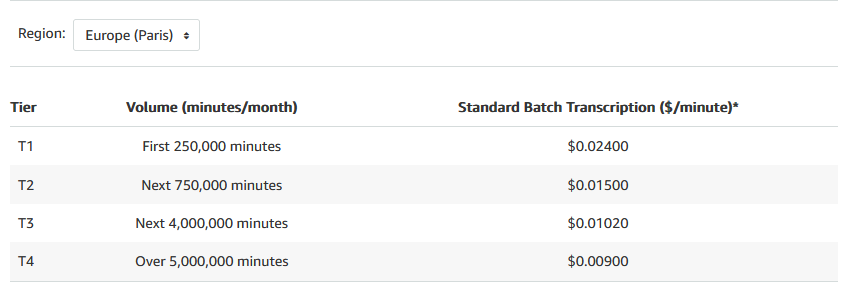
\includegraphics[width=\linewidth*3/4]{graphics/AmazonTranscribePricing.png}
    \caption{Prijzen Amazon Transcribe voor Parijse server \autocite{Amazon2023}}
    \label{fig:PricingAmazonTranscribe}
\end{figure}

\subsection{Microsoft Azure Speech Services}%

\paragraph{\IfLanguageName{dutch}{Beschrijving}{Description}}
Microsoft Azure Speech Services is een spraakherkenningsservice die wordt aangeboden door Microsoft Azure, het cloudplatform van Microsoft.

\paragraph{\IfLanguageName{dutch}{Functies}{Features}}
Azure Speech Services biedt een breed scala aan functies voor spraakherkenning en tekst-naar-spraak-conversie. Enkele van de belangrijkste functies zijn:

\begin{itemize}
    \item \textbf{Spraakherkenning}: De service kan gesproken taal detecteren en omzetten naar tekst in meer dan 60 talen. Het ondersteunt zowel real-time verwerking als batchverwerking van audiobestanden.

    \item \textbf{Taalherkenning}: Azure Speech Services kan automatisch de gesproken taal detecteren, waardoor het mogelijk is om meertalige spraakherkenning te realiseren zonder voorafgaande taalconfiguratie.

    \item \textbf{Aanpassing van modellen}: Gebruikers kunnen de spraakherkenning verbeteren en aanpassen aan specifieke vocabulaires en domeinen door aangepaste taalmodellen te maken. Hierdoor kunnen ze de nauwkeurigheid van de herkenning verhogen voor gespecialiseerde toepassingen.

    \item \textbf{Real-time streaming}: Azure Speech Services ondersteunt real-time streaming van spraak naar tekst, wat ideaal is voor toepassingen zoals live ondertiteling, spraakgestuurde opdrachten en interactieve dialoogsystemen.

    \item \textbf{Text-to-speech}: Naast spraakherkenning biedt de service ook mogelijkheden voor tekst-naar-spraak-conversie. Gebruikers kunnen tekst invoeren en de service genereert menselijke spraakuitvoer in verschillende stemmen en talen.
\end{itemize}

\paragraph{\IfLanguageName{dutch}{Tarieven}{Pricing}}
Per maand bied Azure vijf uur gratis aan daarna moet er een vergoeding van €0,935 betaald worden per uur.

\subsection{Mozilla DeepSpeech}%

\paragraph{\IfLanguageName{dutch}{Beschrijving}{Description}}
In tegenstelling tot de voorgaande services is DeepSpeech van Mozilla open source.

\paragraph{\IfLanguageName{dutch}{Functies}{Features}}
Mozilla DeepSpeech biedt verschillende functies en mogelijkheden voor spraakherkenning. Enkele van de belangrijkste kenmerken zijn:

\begin{itemize}
    \item \textbf{Hoge nauwkeurigheid:} DeepSpeech streeft naar hoge nauwkeurigheid in spraakherkenning en heeft aanzienlijke vooruitgang geboekt in termen van herkenningsscores.

    \item \textbf{Flexibiliteit:} Het systeem kan worden aangepast en afgestemd op specifieke toepassingen of vocabulaires. Hierdoor kan het worden gebruikt voor uiteenlopende spraakherkenningsscenario's.

    \item \textbf{Real-time verwerking:} DeepSpeech is ontworpen om spraak in realtime om te zetten, wat betekent dat het geschikt is voor toepassingen die onmiddellijke spraak-naar-tekstfunctionaliteit vereisen.

    \item \textbf{Privacy:} Als open-sourceproject stelt DeepSpeech gebruikers in staat om spraakherkenningssystemen lokaal uit te voeren, waardoor de privacy van gebruikersinformatie beter gewaarborgd is.
\end{itemize}

\paragraph{\IfLanguageName{dutch}{Tarieven}{Pricing}}
Aangezien dat de service open source is, moet er geen vast tarief betaald worden voor de service. Er kunnen echter wel kosten komen om de service te hosten.

\subsection{Whisper}%

\paragraph{\IfLanguageName{dutch}{Beschrijving}{Description}}
Whisper is de ASR service gemaakt door OpenAI. Het is beschikbaar als een API die ontwikkelaars kunnen integreren in hun eigen toepassingen en systemen door er spraakopnamen naar te sturen. De API geeft vervolgens een tekstuele weergave van de spraak terug als respons.

\paragraph{\IfLanguageName{dutch}{Functies}{Features}}
Whisper heeft verschillende kenmerken en mogelijkheden die het tot een krachtig spraakherkenningssysteem maken:

\begin{itemize}
    \item \textbf{Hoge nauwkeurigheid:} Whisper heeft aanzienlijke vooruitgang geboekt in termen van spraakherkenningsscores en streeft naar hoge nauwkeurigheid bij het omzetten van spraak naar tekst.

    \item \textbf{Meertaligheid:} Het model van Whisper ondersteunt meerdere talen, waardoor het geschikt is voor wereldwijde toepassingen en gebruikers met verschillende taalvereisten.

    \item \textbf{Flexibiliteit:} Whisper kan worden aangepast en afgestemd op specifieke toepassingen en vocabulaires, waardoor het kan worden gebruikt in uiteenlopende spraakherkenningsscenario's.

    \item \textbf{Real-time verwerking:} Het systeem is ontworpen om spraak in realtime te verwerken, wat betekent dat het geschikt is voor toepassingen die onmiddellijke spraak-naar-tekstfunctionaliteit vereisen.

    \item \textbf{Privacy:} OpenAI hanteert strenge beveiligings- en privacyrichtlijnen om de gebruikersgegevens te beschermen. Whisper stelt gebruikers in staat om spraakherkenningssystemen lokaal uit te voeren, waardoor de privacy van gebruikersinformatie beter gewaarborgd is.
\end{itemize}

\paragraph{\IfLanguageName{dutch}{Tarieven}{Pricing}}
Net als Mozilla's DeepSpeech is Whisper open source. Dit betekent dat de kosten afhangen van waar en hoe de service wordt gehost.

\subsection{Kaldi ASR}

\paragraph{\IfLanguageName{dutch}{Beschrijving}{Description}}
Kaldi ASR is een open-source spraakherkenningssysteem dat algemeen wordt gebruikt in de academische wereld en de industrie. Het is ontwikkeld door het Kaldi-project, een community-gedreven initiatief dat zich richt op het leveren van state-of-the-art spraaktechnologie.

Kaldi maakt gebruik van geavanceerde algoritmen en technieken, waaronder deep neural networks (DNN's) en hidden Markov models (HMM's), om spraak naar tekst om te zetten. Het biedt een flexibel en configureerbaar framework dat kan worden aangepast aan verschillende spraakherkenningstoepassingen.

\paragraph{\IfLanguageName{dutch}{Functies}{Features}}
Kaldi ASR biedt een breed scala aan functies en mogelijkheden die het tot een krachtig spraakherkenningssysteem maken:

\begin{itemize}
    \item \textbf{Hoge nauwkeurigheid:} Kaldi is bekend om zijn hoge nauwkeurigheid in spraakherkenning. Het maakt gebruik van geavanceerde modellen en trainingstechnieken om nauwkeurige resultaten te leveren.

    \item \textbf{Flexibiliteit:} Het Kaldi-framework is zeer configureerbaar en aanpasbaar. Het stelt gebruikers in staat om modellen en akoestische kenmerken aan te passen aan specifieke toepassingen en datasets.

    \item \textbf{Meertaligheid:} Kaldi ondersteunt meerdere talen en kan worden gebruikt voor spraakherkenning in verschillende taalomgevingen.

    \item \textbf{Uitgebreide toolkit:} Kaldi wordt geleverd met een uitgebreide toolkit die verschillende hulpmiddelen en utilities biedt voor spraakdataverwerking, modeltraining en evaluatie.

    \item \textbf{Community-ondersteuning:} Het Kaldi-project wordt ondersteund door een actieve gemeenschap van ontwikkelaars en onderzoekers, wat resulteert in regelmatige updates, bugfixes en nieuwe functies.
\end{itemize}

\paragraph{\IfLanguageName{dutch}{Gebruik en implementatie}{Usage and implementation}}
Kaldi ASR wordt meestal gebruikt via de command line-interface en vereist enige technische kennis om effectief te kunnen gebruiken. Het proces om Kaldi te gebruiken omvat het verzamelen en voorbereiden van spraakgegevens, het trainen van akoestische en taalmodellen, en het uitvoeren van de spraakherkenning op nieuwe gegevens.

Kaldi biedt documentatie en handleidingen om gebruikers te begeleiden bij de implementatie en het gebruik van het systeem. Het heeft een actieve gebruikersgemeenschap waar gebruikers vragen kunnen stellen en ervaringen kunnen delen.

\paragraph{\IfLanguageName{dutch}{Beschikbaarheid en prijs}{Availability and pricing}}
Kaldi ASR is een open-source project en is vrij beschikbaar voor iedereen. Het kan worden gedownload van de officiële Kaldi-website en lokaal worden uitgevoerd.


\section{\IfLanguageName{dutch}{Natuurlijke taalverwerking}{Natural Language Classifier}} \label{sec:Natural Language Classifier}%

\subsection{GPT series}%

\paragraph{\IfLanguageName{dutch}{Beschrijving}{Description}}
The GPT, wat staat voor Generative Pre-trained Transformer, series zijn algemene taalmodellen gemaakt door OpenAI. Het doel van deze modellen is genereren van menselijke taal op basis van de gegeven input. Het meest bekende voorbeeld is OpenAI's chatbot, ChatGPT. Het  maakt gebruik van GPT-3.5 en GPT-4 om antwoorden te genereren. Deze modellen zijn getraind op een brede set van internet data.

\paragraph{\IfLanguageName{dutch}{Tarieven}{Pricing}}
Er zijn twee GPT-4 modellen beschikbaar de 8K context en de 32K context. Om ze te gebruiken moet er betaald worden per 1000 tokens. Dat is ongeveer gelijk aan 750 woorden. Voor de 8K context is de prijs \$0.03 voor invoer en \$0.06 voor de uitvoer. De kost voor 32K context is \$0.06 voor invoer en \$0.12 voor het resultaat. Afhankelijk van het model is de prijs voor GPT-3 tussen de \$0.0004 of \$0.02 per 1000 tokens.

\subsection{BERT}%

\paragraph{\IfLanguageName{dutch}{Beschrijving}{Description}}
BERT, wat staat voor Bidirectional Encoder Representations from Transformers, is een ander type taalmodel ontwikkeld door Google AI Language. In tegenstelling tot de GPT-series, is BERT een bi-richtingstransformer, wat betekent dat het in staat is om zowel de context vóór als na een woord te begrijpen tijdens het trainen.

\paragraph{\IfLanguageName{dutch}{Tarieven}{Pricing}}
In tegenstelling tot de GPT reeks is BERT gratis te gebruiken. Het taalmodel vereist wel aanzienlijke rekenkracht en geheugen waardoor de hardware waarop het draait sterk genoeg moet zijn.

\subsection{FlairNLP}%

\paragraph{\IfLanguageName{dutch}{Beschrijving}{Description}}
FlairNLP is een NLP (Natural Language Processing) framework ontwikkeld door Zalando Research. Het staat voor "Flexible Language-Agnostic IRst-order" en is gericht op het bieden van flexibiliteit en veelzijdigheid in het verwerken van natuurlijke taal. Net als BERT en GPT maakt FlairNLP gebruik van transformer-gebaseerde modellen en kan worden gebruikt voor een breed scala aan taalverwerkings-taken.

\paragraph{\IfLanguageName{dutch}{Tarieven}{Pricing}}
Ook FlairNLP is open-source wat wil zeggen dat de kosten afhangen van hoe en waar de software op draait.

\subsection{RoBERTa}%

\paragraph{\IfLanguageName{dutch}{Beschrijving}{Description}}
RoBERTa staat voor "A Robustly Optimized BERT Pretraining Approach." Het is een door Meta AI ontwikkelde transformer-gebaseerd taalmodel en een doorontwikkeling van BERT. RoBERTa is ontworpen om de prestaties van BERT verder te verbeteren door middel van optimalisaties in de trainingsprocedure.

In tegenstelling tot BERT maakt RoBERTa gebruik van een grotere hoeveelheid trainingsdata en een langere trainingsduur, wat het model helpt om een dieper taalbegrip te ontwikkelen. Het trainingsproces van RoBERTa omvat het maskeren van woorden in een zin en het uitdagen van het model om de ontbrekende woorden correct te voorspellen, vergelijkbaar met BERT.

\paragraph{\IfLanguageName{dutch}{Tarieven}{Pricing}}
RoBERTa is net als BERT gratis te gebruiken.


%Dit hoofdstuk bevat je literatuurstudie. De inhoud gaat verder op de inleiding, maar zal het onderwerp van de bachelorproef *diepgaand* uitspitten. De bedoeling is dat de lezer na lezing van dit hoofdstuk helemaal op de hoogte is van de huidige stand van zaken (state-of-the-art) in het onderzoeksdomein. Iemand die niet vertrouwd is met het onderwerp, weet nu voldoende om de rest van het verhaal te kunnen volgen, zonder dat die er nog andere informatie moet over opzoeken \autocite{Pollefliet2011}.
%
%Je verwijst bij elke bewering die je doet, vakterm die je introduceert, enz.\ naar je bronnen. In \LaTeX{} kan dat met het commando \texttt{$\backslash${textcite\{\}}} of \texttt{$\backslash${autocite\{\}}}. Als argument van het commando geef je de ``sleutel'' van een ``record'' in een bibliografische databank in het Bib\LaTeX{}-formaat (een tekstbestand). Als je expliciet naar de auteur verwijst in de zin, gebruik je \texttt{$\backslash${}textcite\{\}}.
%Soms wil je de auteur niet expliciet vernoemen, dan gebruik je \texttt{$\backslash${}autocite\{\}}. In de volgende paragraaf een voorbeeld van elk.
%
%\textcite{Knuth1998} schreef een van de standaardwerken over sorteer- en zoekalgoritmen. Experten zijn het erover eens dat cloud computing een interessante opportuniteit vormen, zowel voor gebruikers als voor dienstverleners op vlak van informatietechnologie~\autocite{Creeger2009}.
%
%\lipsum[7-20]

%%=============================================================================
%% Methodologie
%%=============================================================================

\chapter{\IfLanguageName{dutch}{Methodologie}{Methodology}}%
\label{ch:methodologie}

%% TODO: Hoe ben je te werk gegaan? Verdeel je onderzoek in grote fasen, en
%% licht in elke fase toe welke stappen je gevolgd hebt. Verantwoord waarom je
%% op deze manier te werk gegaan bent. Je moet kunnen aantonen dat je de best
%% mogelijke manier toegepast hebt om een antwoord te vinden op de
%% onderzoeksvraag.

%\lipsum[21-25]

Dit onderzoek start met een literatuurstudie (\ref{chap:State of the art}). Vervolgens wordt er een requirementsanalyse gehouden waar gekeken wordt wat er van de oplossing verwacht wordt (\ref{sect:Requirements analysis}). Na de requirements vast te leggen zullen verschillende spraak naar tekst software (\ref{sect:Speech to text}) en taalverwerkingsmodellen (\ref{sect:Language models}) getest worden. Als laatste zal er een proof-of-concept opgesteld worden.

\section{\IfLanguageName{dutch}{Requirementsanalyse}{Requirements analysis}} \label{sect:Requirements analysis}%

De requirementsanalyse start met een opsomming van functionele en niet-functionele requirements. Vervolgens worden ze aan de hand van de MoSCoW methode gerangschikt op relevantie. Als laatste wordt er een use case opgesteld.

\subsection{\IfLanguageName{dutch}{Functionele requirements}{Functional requirements}}

\begin{itemize}
    \item De applicatie moet in staat zijn om spraak te herkennen en te registreren hoelang en tot wanneer de gebruiker spreekt.
    \item De applicatie moet in staat zijn om de gesproken woorden om te zetten in tekst, zodat deze kunnen worden opgeslagen en verwerkt.
    \item De applicatie moet in staat zijn om op basis van de gegenereerde tekst een volgend fragment te kiezen dat aansluit bij het onderwerp en de context van de tekst.
    \item De applicatie moet gebruik maken van AI-technieken om spraakherkenning en tekstgeneratie mogelijk te maken.
    \item De applicatie moet gemakkelijk te gebruiken zijn voor de gebruiker, zonder dat deze technische kennis nodig heeft.
    \item De applicatie moet betrouwbaar zijn en weinig tot geen fouten maken bij het herkennen van spraak en genereren van tekst.
    \item  De applicatie moet in staat zijn om de opgeslagen tekst te doorzoeken op bepaalde trefwoorden of zinnen, om zo snel specifieke informatie te kunnen vinden.
    \item De applicatie moet aanpasbaar zijn aan de specifieke wensen en behoeften van de gebruiker, zoals het leren herkennen van patronen in gebruikers met een spraakbeperking.
\end{itemize}

\subsection{\IfLanguageName{dutch}{Niet-functionele requirements}{Non-functional requirements}}

\begin{itemize}
    \item Nauwkeurigheid: De spraakherkenningssoftware moet zeer nauwkeurig zijn bij het herkennen en transcriberen van spraak, omdat eventuele fouten kunnen leiden tot onnauwkeurige resultaten en mogelijk onjuiste interpretaties.
    \item Snelheid: De software moet snel genoeg zijn om de spraak te herkennen en te transcriberen, zodat het in real-time kan werken en niet leidt tot onnodige vertragingen of onderbrekingen.
    \item Veiligheid: De privacy en veiligheid van de gebruiker moeten worden beschermd, zodat de spraakgegevens niet kunnen worden gehackt of gelekt.
\end{itemize}

\subsection{\IfLanguageName{dutch}{MoSCoW}{MoSCoW}}%

Aan de hand van de MoSCoW methode bepalen we het belang van verschillende functionaliteiten.

\begin{enumerate}
    \item Must have:
    \begin{itemize}
        \item De applicatie moet in staat zijn om de gesproken woorden om te zetten in tekst, zodat deze kunnen worden opgeslagen en verwerkt.
        \item De applicatie moet in staat zijn om op basis van de gegenereerde tekst een volgend fragment te kiezen dat aansluit bij het onderwerp en de context van de tekst.
        \item De applicatie moet gebruik maken van AI-technieken om spraakherkenning en tekstgeneratie mogelijk te maken.
        \item  De applicatie moet in staat zijn om de opgeslagen tekst te doorzoeken op bepaalde trefwoorden of zinnen, om zo snel specifieke informatie te kunnen vinden.
    \end{itemize}
    \item Should have:
    \begin{itemize}
        \item De applicatie moet in staat zijn om spraak te herkennen en te registreren hoelang en tot wanneer de gebruiker spreekt.
        \item De applicatie moet gemakkelijk te gebruiken zijn voor de gebruiker, zonder dat deze technische kennis nodig heeft.
        \item De applicatie moet betrouwbaar zijn en weinig tot geen fouten maken bij het herkennen van spraak en genereren van tekst.
    \end{itemize}
    \item Could have:
    \begin{itemize}
        \item De applicatie moet aanpasbaar zijn aan de specifieke wensen en behoeften van de gebruiker, zoals het leren herkennen van patronen in gebruikers met een spraakbeperking.
        \item Een flexibel systeem met verschillende scenario’s creëren
    \end{itemize}
\end{enumerate}

\subsection{\IfLanguageName{dutch}{Use Case}{Use case}}%




\section{\IfLanguageName{dutch}{Proof-of-concept}{Proof-of-concept}} \label{sect:Proof-of-concept}%

dfsdfsd

% Voeg hier je eigen hoofdstukken toe die de ``corpus'' van je bachelorproef
% vormen. De structuur en titels hangen af van je eigen onderzoek. Je kan bv.
% elke fase in je onderzoek in een apart hoofdstuk bespreken.

%\input{...}
%\input{...}
%...

%%=============================================================================
%% Conclusie
%%=============================================================================

\chapter{Conclusie}%
\label{ch:conclusie}

% TODO: Trek een duidelijke conclusie, in de vorm van een antwoord op de
% onderzoeksvra(a)g(en). Wat was jouw bijdrage aan het onderzoeksdomein en
% hoe biedt dit meerwaarde aan het vakgebied/doelgroep?
% Reflecteer kritisch over het resultaat. In Engelse teksten wordt deze sectie
% ``Discussion'' genoemd. Had je deze uitkomst verwacht? Zijn er zaken die nog
% niet duidelijk zijn?
% Heeft het onderzoek geleid tot nieuwe vragen die uitnodigen tot verder
%onderzoek?

Het onderzoek richtte zich op het gebruik van AI om stotterpatiënten een meer interactieve ervaring te bieden door spraakherkenningstechnologie toe te passen. De onderzoeksvragen waren gericht op het registreren van spraak, potentiële problemen bij spraakregistratie, de invloed van stotteraspecten op spraakherkenning en hoe de applicatie volgende spraakfragmenten kiest op basis van gegenereerde tekst.

Uit de literatuurstudie kwamen verschillende obstakels aan bod zoals domeinproblemen, natuurlijke taalverwerking problemen en de efficiëntie van de apparatuur. Aangezien de fragmenten bestonden uit video's van het Nederlandse YouTube kanaal 'StotterFonds', was er van achtergrond lawaai en meerdere sprekers geen probleem. Ook de taal en dialecten gaven geen moeilijkheid hoewel er geen duidelijkheid is hoe Belgisch Nederlands een verschil kan maken. Het domein waarin de modellen getraind zijn en de use case komen daarentegen niet overeen. De gebruikte modellen zijn gedoeld voor alledaags Nederlands en niet getraind op stotteren. De aanwezige obstakels bij de spraakherkenning van stottermomenten zijn vooral het herhalen van woorden en de blokkeringen. Deze zorgen ervoor dat de ASR de haperingen wilt registreren als aparte woorden of het woord meermaals achter elkaar zet. Dit was vooral op te vallen bij Azure.

De spraak wordt in de POC applicatie aan de hand van het gekozen invoerapparaat geregistreerd via een vooraf gekozen push-to-talk toets. Waarna het gecreëerde audiofragment met het gekozen model wordt verwerkt. Op basis van de resultaten blijkt het medium model van Whisper de beste optie voor het transcriberen van stotterpatiënten. Zo blijft de tijd en nauwkeurigheid van het model consistent over de fragmenten heen hoewel de duur wat langer is dan het Azure en kleine Whisper model. Die modellen hebben echter een hogere WER, vooral bij stotterfragmenten. Google is daarentegen uitgesloten dankzij de lange tijd die het neemt om een fragment te verwerken. Als laatste is het kiezen van een vervolg fragment op basis van wat de spreker antwoord is niet tot stand gekomen binnen de tweede examenperiode.

De uitslag van dit onderzoek had ik niet verwacht. Zo veronderstelde ik op voorhand dat de betaalde services van Google of Microsoft de bovenhand zouden hebben tegenover de open source Whisper. Ik wist dat de open source community niet te onderschatten was met de vele bijdragers maar toch dacht ik dat de grote namen beter zouden presteren. Daarnaast ben ik teleurgesteld in mezelf en vind ik het jammer dat ik er niet in ben geslaagd om het kiezen van een vervolg fragment te realiseren.

Aangezien dit onderzoek was uitgevoerd in het kader van het 360° Zorglab, bieden de resultaten een meerwaarde. Hopelijk kunnen ze aan de hand van de cijfers en de POC verdere ideeën uitwerken om effectief toe te passen in hun stottertherapie of andere doeleinden. Ook kan deze paper als basis gebruikt worden om verder onderzoek naar spraakherkenning van stotterpatiënten uit te voeren of om het schakelen van fragmenten uit te werken en te implementeren. Zo kan er mogelijks onderzoek gedaan worden naar hoe het Zorglab zelf een model kan maken met de data die ze in hun sessies verzamelen.



%---------- Bijlagen -----------------------------------------------------------

\appendix

\chapter{Onderzoeksvoorstel}

Het onderwerp van deze bachelorproef is gebaseerd op een onderzoeksvoorstel dat vooraf werd beoordeeld door de promotor. Dat voorstel is opgenomen in deze bijlage.

%% TODO:
%\section*{Samenvatting}

% Kopieer en plak hier de samenvatting (abstract) van je onderzoeksvoorstel.

% Verwijzing naar het bestand met de inhoud van het onderzoeksvoorstel
%---------- Inleiding ---------------------------------------------------------

\section{Introductie}%
\label{sec:introductie}

In de reclamespot `The Impact Will Be Real` over de Metaverse toont \textcite{Meta2022} hun visie over de rol die Virtual Reality (VR) speelt in de toekomst. Zo laten ze verschillende toepassingen ervan in het onderwijs zien. Jammer genoeg staat onze technologie nog niet zo ver als wat er in de reclame gezien kan worden maar ook nu al vindt VR zich een baan in verschillende opleidingen.

De Hogeschool van Gent maakt ook gebruik van VR om studenten de kans te geven in meer realistische situaties te oefenen. Hiervoor zijn twee verschillende technieken gebruikt. Allereerst heb je het renderen van een omgeving. Dit laat de gebruiker een interactieve wereld van 3D modellen ontdekken. Zo bestaan er drie virtuele kamers waarin de student kan oefenen. De andere manier is aan de hand van een 360° opname die wordt gemaakt aan de hand van een 360° camera. Omdat dit een opname van de werkelijkheid neemt, ziet deze methode er realistischer uit.

Dit is waar er op het probleem wordt gestoten. Aangezien de tweede methode werkt met een opname moet er naar verschillende fragmenten gesprongen worden naargelang het antwoord dat de gebruiker ingeeft. Dit wordt handmatig gedaan via een meerkeuzevraag. Hierdoor staat de oefening tijdelijk stil wat de echtheid van de situatie weghaalt. Daarom wordt in deze bachelorproef toegepaste informatica onderzocht hoe het overschakelen anders kan aangepakt worden zodat het voor de gebruiker realistischer aanvoelt. Hiervoor kijken we richting Artificiële Intelligentie (AI).

Alle grote IT bedrijven hebben wel een departement die zich bezighoudt met AI. Ze zien allemaal de mogelijkheden die het biedt. Van jobs gemakkelijker te maken tot het zelf creëren van kunst, de toepassingen zijn oneindig. Daarom zal in functie van het Zorglab op zoek worden gegaan naar een Spraak naar tekst (STT) en een natuurlijke taalverwerking software (NLP).

De STT zal worden gebruikt om het manueel ingeven van het antwoord te vervangen. In plaats daarvan zal de gebruiker gewoon zijn antwoord luidop kunnen geven en zal de STT dit in tekst omzetten. Dit alleen zal natuurlijk geen volgend fragment voor de gebruiker kunnen kiezen en daarom hebben we de NLP nodig. Deze zal de gegenereerde tekst omzetten naar kernwoorden en aan de hand daarvan bepalen welk fragment als volgende geschikt is.



% Waarover zal je bachelorproef gaan? Introduceer het thema en zorg dat volgende zaken zeker duidelijk aanwezig zijn:
%
%\begin{itemize}
%  \item kaderen thema
%  \item de doelgroep
%  \item de probleemstelling en (centrale) onderzoeksvraag
%  \item de onderzoeksdoelstelling
%\end{itemize}
%
%Denk er aan: een typische bachelorproef is \textit{toegepast onderzoek}, wat betekent dat je start vanuit een concrete probleemsituatie in bedrijfscontext, een \textbf{casus}. Het is belangrijk om je onderwerp goed af te bakenen: je gaat voor die \textit{ene specifieke probleemsituatie} op zoek naar een goede oplossing, op basis van de huidige kennis in het vakgebied.
%
%De doelgroep moet ook concreet en duidelijk zijn, dus geen algemene of vaag gedefinieerde groepen zoals \emph{bedrijven}, \emph{developers}, \emph{Vlamingen}, enz. Je richt je in elk geval op it-professionals, een bachelorproef is geen populariserende tekst. Eén specifiek bedrijf (die te maken hebben met een concrete probleemsituatie) is dus beter dan \emph{bedrijven} in het algemeen.
%
%Formuleer duidelijk de onderzoeksvraag! De begeleiders lezen nog steeds te veel voorstellen waarin we geen onderzoeksvraag terugvinden.
%
%Schrijf ook iets over de doelstelling. Wat zie je als het concrete eindresultaat van je onderzoek, naast de uitgeschreven scriptie? Is het een proof-of-concept, een rapport met aanbevelingen, \ldots Met welk eindresultaat kan je je bachelorproef als een succes beschouwen?

%---------- Stand van zaken ---------------------------------------------------

\section{State-of-the-art}%
\label{sec:state-of-the-art}

Om de immersie in de simulatie te vergroten moet ervoor gezorgd worden dat het overschakelen naar een volgend fragment kan gebeuren zonder de gebruiker uit de illusie te halen. Hiervoor zouden verbale antwoorden gegeven kunnen worden.

Een mooi voorbeeld van zo een interactie is het project 'Dimensions in Testimony' van de \textcite{USCShoahFoundation2020}. Daar kunnen bezoekers vragen stellen aan een overlevende van de Holocaust die op voorhand een volledig interview heeft afgelegd. Dit werd mogelijk gemaakt dankzij het systeem dat erachter zit (Figuur \ref{fig:DiTArchitecture}). Dit systeem is opgebouwd uit volgende componenten: een software voor spraakherkenning (ASR) die de gebruikers verbale vraag in tekst omzet, een Natural Language Classifier (NLC) die op basis van de gegenereerde tekst een antwoord via een audio/video fragment voorziet en een mediaspeler die de fragmenten kan afspelen met tussendoor een inactieve animatie \autocite{Traum2015}.

\begin{figure}[h]
    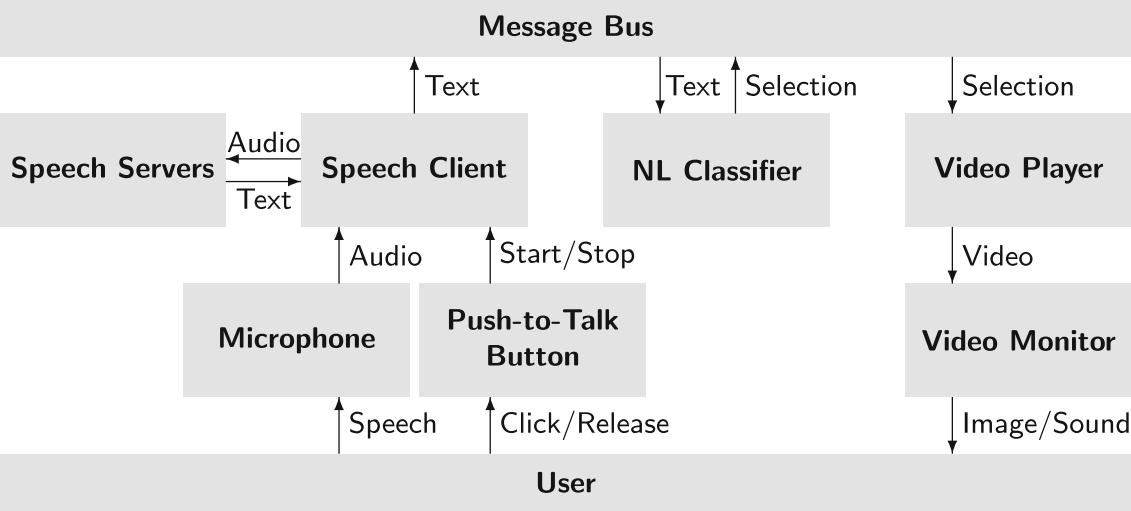
\includegraphics[width=\linewidth]{TraumDEtAl_DimensionsInTestimony_SystemArchitecture.png}
    \caption{Dimensions in Testimony - Systeem Architectuur \autocite{Traum2015}}
    \label{fig:DiTArchitecture}
\end{figure}

Spraakherkenning is de laatste jaren veel vooruitgegaan, dit komt omdat er meer data beschikbaar is, de algoritmes beter (deep neural networks) en de computers sneller zijn. Maar perfect zullen ze nooit zijn zegt \textcite{Hessen2020}. Dit is geen verrassing aangezien mensen zelf vaak nog problemen hebben bij het verstaan van een andere. De meest voorkomende fouten van een ASR zijn herkenningsfouten. Deze kunnen ontstaan door slechte kwaliteit van de opname maar ook van de manier waarop woorden worden uitgesproken. De andere fouten ontstaan omdat ASR zijn vocabulaire niet uitgebreid genoeg is. Dit noemen we Out-of-vocabulary-fouten (OOV) \autocite{Hessen2020}.

Naast de ASR hebben we ook de natuurlijke taalverwerking (NLP). In 'Dimension in Testimony' maakten ze hiervoor gebruik van NCPEditor (Figuur \ref{fig:NPCEArchitecture}). De classifier in dit systeem berekent welke antwoorden op de ingegeven tekst kunnen gegeven worden door de taalmodellen van beide te vergelijken en de antwoorden te rangschikken. Zolang de ingegeven tekst een foutmarge lager dan 50\% blijft, zal het antwoord ongewijzigd blijven \autocite{Leuski2010}.

\begin{figure}[h]
    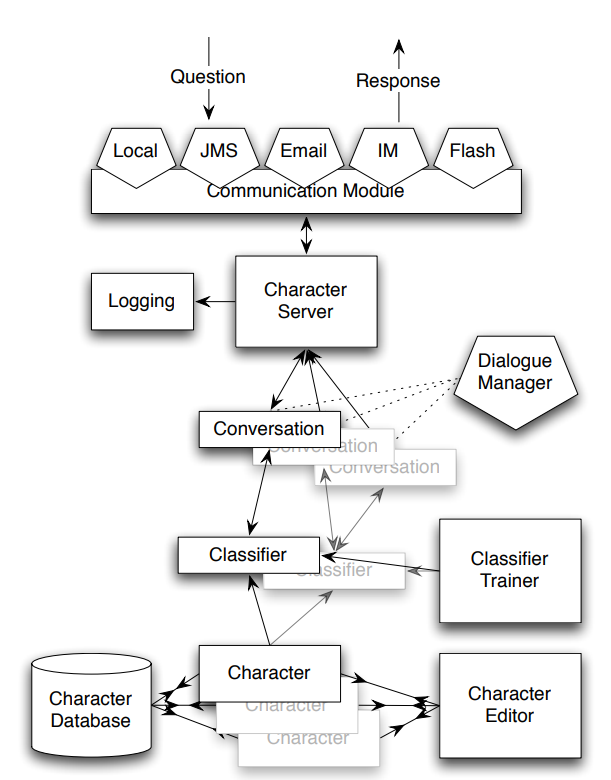
\includegraphics[width=\linewidth]{Traum&Leuski_NPCEditor_System architecture.png}
    \caption{NPCEditor - Systeem Architectuur \autocite{Leuski2010}}
    \label{fig:NPCEArchitecture}
\end{figure}

%Hier beschrijf je de \emph{state-of-the-art} rondom je gekozen onderzoeksdomein, d.w.z.\ een inleidende, doorlopende tekst over het onderzoeksdomein van je bachelorproef. Je steunt daarbij heel sterk op de professionele \emph{vakliteratuur}, en niet zozeer op populariserende teksten voor een breed publiek. Wat is de huidige stand van zaken in dit domein, en wat zijn nog eventuele open vragen (die misschien de aanleiding waren tot je onderzoeksvraag!)?
%
%Je mag de titel van deze sectie ook aanpassen (literatuurstudie, stand van zaken, enz.). Zijn er al gelijkaardige onderzoeken gevoerd? Wat concluderen ze? Wat is het verschil met jouw onderzoek?
%
%Verwijs bij elke introductie van een term of bewering over het domein naar de vakliteratuur, bijvoorbeeld~\autocite{Hykes2013}! Denk zeker goed na welke werken je refereert en waarom.
%
%Draag zorg voor correcte literatuurverwijzingen! Een bronvermelding hoort thuis \emph{binnen} de zin waar je je op die bron baseert, dus niet er buiten! Maak meteen een verwijzing als je gebruik maakt van een bron. Doe dit dus \emph{niet} aan het einde van een lange paragraaf. Baseer nooit teveel aansluitende tekst op eenzelfde bron.
%
%Als je informatie over bronnen verzamelt in JabRef, zorg er dan voor dat alle nodige info aanwezig is om de bron terug te vinden (zoals uitvoerig besproken in de lessen Research Methods).

% Voor literatuurverwijzingen zijn er twee belangrijke commando's:
% \autocite{KEY} => (Auteur, jaartal) Gebruik dit als de naam van de auteur
%   geen onderdeel is van de zin.
% \textcite{KEY} => Auteur (jaartal)  Gebruik dit als de auteursnaam wel een
%   functie heeft in de zin (bv. ``Uit onderzoek door Doll & Hill (1954) bleek
%   ...'')

%Je mag deze sectie nog verder onderverdelen in subsecties als dit de structuur van de tekst kan verduidelijken.

%---------- Methodologie ------------------------------------------------------
\section{Methodologie}%
\label{sec:methodologie}

Om te beginnen zal er worden samengezeten met het team van het Zorglab om een requirementsanalyse uit te voeren. Zo kan worden neergeschreven wat de problemen zijn en waar ze tegenaan lopen. Ook wordt daarin besproken aan de hand van de MoSCoW methode wat er verwacht wordt van een oplossing, hoe moet deze in zijn werk gaan? Op basis daarvan zal de literatuurstudie uitgebreid worden met onderzoek naar oplossingen die dit probleem kunnen verhelpen. Hieronder valt onder andere een onderzoek naar ASR. Er zal gekeken worden welke ASR's er al verkrijgbaar zijn en welke er in het Nederlands werken. Alleen een ASR hebben is niet genoeg om de immersie te behouden dus zal er ook worden gekeken naar hoe, aan de hand van de gegenereerde tekst, het volgende fragment getoond kan worden.

Wanneer er een uitgebreide literatuurstudie is uitgevoerd, zal een proof of concept opgesteld worden. Hierin wordt de software die gevonden is op de proef gesteld. Hier wordt gekeken hoe correct de ASR's inkomende audio kunnen transcriberen. Daarnaast zal ook getest worden of er aan de hand van kernwoorden een juist fragment gekozen kan worden. Door de AI verschillende prompts te geven en te kijken of hij naar de juiste tijdsaanduiding in de video gaat. Nadat de poc afgewerkt is, wordt deze beoordeelt om te kijken hoe het in de context van het Zorglab toegepast kan worden.

%Hier beschrijf je hoe je van plan bent het onderzoek te voeren. Welke onderzoekstechniek ga je toepassen om elk van je onderzoeksvragen te beantwoorden? Gebruik je hiervoor literatuurstudie, interviews met belanghebbenden (bv.~voor requirements-analyse), experimenten, simulaties, vergelijkende studie, risico-analyse, PoC, \ldots?
%
%Valt je onderwerp onder één van de typische soorten bachelorproeven die besproken zijn in de lessen Research Methods (bv.\ vergelijkende studie of risico-analyse)? Zorg er dan ook voor dat we duidelijk de verschillende stappen terug vinden die we verwachten in dit soort onderzoek!
%
%Vermijd onderzoekstechnieken die geen objectieve, meetbare resultaten kunnen opleveren. Enquêtes, bijvoorbeeld, zijn voor een bachelorproef informatica meestal \textbf{niet geschikt}. De antwoorden zijn eerder meningen dan feiten en in de praktijk blijkt het ook bijzonder moeilijk om voldoende respondenten te vinden. Studenten die een enquête willen voeren, hebben meestal ook geen goede definitie van de populatie, waardoor ook niet kan aangetoond worden dat eventuele resultaten representatief zijn.
%
%Uit dit onderdeel moet duidelijk naar voor komen dat je bachelorproef ook technisch voldoen\-de diepgang zal bevatten. Het zou niet kloppen als een bachelorproef informatica ook door bv.\ een student marketing zou kunnen uitgevoerd worden.
%
%Je beschrijft ook al welke tools (hardware, software, diensten, \ldots) je denkt hiervoor te gebruiken of te ontwikkelen.
%
%Probeer ook een tijdschatting te maken. Hoe lang zal je met elke fase van je onderzoek bezig zijn en wat zijn de concrete \emph{deliverables} in elke fase?

%---------- Verwachte resultaten ----------------------------------------------
\section{Verwacht resultaat, conclusie}%
\label{sec:verwachte_resultaten}

Uit deze bachelorproef wordt verwacht dat er een proof of concept opgesteld wordt. Hierin zal gekeken zijn of het haalbaar is om aan de hand van spraakherkenning en natuurlijke taalverwerking software een slecht nieuws gesprek oefening, in het Zorglab, vlotter te doen verlopen. Zo kan het Zorglab kiezen of ze dit idee effectief aan het lab willen toevoegen. Dit kan dan aan de hand van de software dat in het PoC is gebruikt. Anderzijds kunnen ze op basis ervan andere software met hetzelfde doeleinde inzetten.

%Hier beschrijf je welke resultaten je verwacht. Als je metingen en simulaties uitvoert, kan je hier al mock-ups maken van de grafieken samen met de verwachte conclusies. Benoem zeker al je assen en de onderdelen van de grafiek die je gaat gebruiken. Dit zorgt ervoor dat je concreet weet welk soort data je moet verzamelen en hoe je die moet meten.
%
%Wat heeft de doelgroep van je onderzoek aan het resultaat? Op welke manier zorgt jouw bachelorproef voor een meerwaarde?
%
%Hier beschrijf je wat je verwacht uit je onderzoek, met de motivatie waarom. Het is \textbf{niet} erg indien uit je onderzoek andere resultaten en conclusies vloeien dan dat je hier beschrijft: het is dan juist interessant om te onderzoeken waarom jouw hypothesen niet overeenkomen met de resultaten.



%%---------- Andere bijlagen --------------------------------------------------
% TODO: Voeg hier eventuele andere bijlagen toe. Bv. als je deze BP voor de
% tweede keer indient, een overzicht van de verbeteringen t.o.v. het origineel.
%\input{...}

%%---------- Backmatter, referentielijst ---------------------------------------

\backmatter{}

\setlength\bibitemsep{2pt} %% Add Some space between the bibliograpy entries
\printbibliography[heading=bibintoc]

\end{document}
